% =============================================================================
% Lecture 15: Adversarial Verification
% Physical AI: Machine Learning Systems That Sense and Act (Volume IV), Chapter 15
% =============================================================================
% Thesis: the claims that matter describe behavior after a fault, so they are
% tested by injecting the fault on purpose, witnessing the response with
% instruments the fault cannot reach, and scoring it against an oracle fixed
% before the run.
% Hook and synthesis: Bookout v. Toyota, 2013 (War Story 15.1; Barr 2013).
% Running case: fault F1, a proposer stall at the rack end, on the running
% machine (shown as a real machine of its class, an ER-FLEX mobile manipulator).
%
% Build: make deck V=4 D=15_verification   (figures: images/make_figs.py,
%        numbers: images/calcs.py, record: images/make_record.py,
%        run: images/watchdog_run.py)
% Plan:  lecture_map.yml in this folder.
% Numbers: the rendered chapter (illustrative values say so), papers read at
% the table named on the slide; derived values print from images/calcs.py.
% Second lecture later: the natural split falls after the Fault List section
% (chapter section 15.6); see lecture_map.yml, notes_for_author.
% =============================================================================

\documentclass[aspectratio=169, 12pt]{beamer}
\usepackage{../../assets/beamerthememlsys}
\mlsyssetup{
  volume={Volume IV},
  chapter={Chapter 15},
  chaptertitle={Adversarial Verification},
  layer=governance,
  logo={../../assets/img/logo-mlsysbook.png},
  instlogo={../../assets/img/logo-harvard.png},
}
\usepackage[T1]{fontenc}
\usepackage[scaled=0.9]{helvet}
\usepackage{courier}
\renewcommand{\familydefault}{\sfdefault}
\usepackage{booktabs,amsmath,array}
\usetikzlibrary{arrows.meta,positioning}
\graphicspath{{images/}}
% Generated by calcs.py. Do not edit; edit calcs.py and rerun it.
\defval{verdict_musd}{3}
\defval{whisker_ohm}{248}
\defval{v_aisle}{1.3}
\defval{d_clear_mm}{1{,}100}
\defval{d_clear_m}{1.10}
\defval{budget}{969.0}
\defval{spare}{131.0}
\defval{spare_mm0}{131}
\defval{t_spare}{100.8}
\defval{t_da}{63.3}
\defval{travel_da}{82.3}
\defval{spare_left}{48.7}
\defval{t_left}{37.5}
\defval{t_takeover}{605}
\defval{travel_takeover}{786.5}
\defval{takeover_over}{655.5}
\defval{chunk_period}{50}
\defval{bus_nominal}{47.7}
\defval{bus_uvlo}{33}
\defval{dfi_faults}{98{,}400}
\defval{dfi_days}{615}
\defval{dfi_hours}{4}
\defval{dfi_found}{561}
\defval{dfi_hazard}{460}
\defval{dfi_scenes_haz}{68}
\defval{dfi_scenes}{7{,}200}
\defval{dfi_scene_pct}{0.94}
\defval{dfi_random}{5{,}000}
\defval{dfi_gpu}{2{,}400}
\defval{dfi_sdc}{1.9}
\defval{dfi_due}{7.35}
\defval{a_brake}{2}
\defval{mu_knee}{0.204}
\defval{mu_insp}{0.12}
\defval{a_insp}{1.18}
\defval{ceiling_dry}{1.44}
\defval{ceiling_insp}{1.23}
\defval{budget_insp_m}{1.19}
\defval{bus_low}{42}
\defval{stall_ms}{30}
\defval{stall_mm}{39}
\defval{v_restricted}{1}
\defval{tau_delay}{133.6}
\defval{capture_travel}{173.7}
\defval{stop_mm}{605.3}
\defval{loc_margin}{150}
\defval{eps_track}{40}
\defval{onset}{82}
\defval{renewal_travel}{106.6}
\defval{f1_bound}{751.9}
\defval{gap}{217.1}
\defval{t_lease}{60}
\defval{t_tick}{1}
\defval{t_bus}{1}
\defval{t_act}{20}
\defval{j_brake}{7.11}
\defval{sfx_v2}{422.5}
\defval{sfx_jerk}{182.8}
\defval{t_age}{51.6}
\defval{age_travel}{67.1}
\defval{late_equiv}{167}
\defval{f1_restricted}{629.6}
\defval{oracle_cut_pct}{16.3}
\defval{speed_cut_pct}{23.1}
\defval{late_ms}{30}
\defval{late_rho_mm}{1}
\defval{t_cmd}{61}
\defval{t_frame}{62}
\defval{rest_on_time}{1{,}013}
\defval{travel_on_time}{711.9}
\defval{t_probe}{65}
\defval{onset_late}{112}
\defval{travel_late}{750.9}
\defval{rho_onset_n}{0.366}
\defval{rho_dist_n}{0.0013}
\defval{chk_onset}{90}
\defval{chk_rho}{8}
\defval{chk_extra}{10.4}
\defval{i_rail}{70}
\defval{bus_r_mohm}{60}
\defval{bus_r_ohm}{0.060}
\defval{bus_min}{37.8}
\defval{bus_margin}{4.8}
\defval{i_cross}{150}
\defval{r_cross}{129}
\defval{holdup_s}{2}
\defval{flag_to_set}{1{,}313.4}
\defval{flag_path}{22}
\defval{holdup_stop}{1{,}211.4}
\defval{engage}{80}
\defval{holdup_margin}{686.6}
\defval{patch_banana}{97}
\defval{patch_toaster}{99}
\defval{openvla_b}{7}
\defval{wang_low}{54}
\defval{wang_high}{88}
\defval{wang_patched}{zero}
\defval{robopair_n}{35}
\defval{go2_direct}{3}
\defval{go2_pair}{35}
\defval{jackal_direct}{1}
\defval{jackal_pair}{35}
\defval{pair_pct}{100}
\defval{enforcer_deadline}{400}
\defval{side_clearance}{0.15}
\defval{vnn_n}{25}
\defval{vnn_max_m}{138}
\defval{intent_b}{7}
\defval{chunk_m}{80}
\defval{intent_over_vnn}{50.7}
\defval{eps_gap_max}{0.131}
\defval{fit_sensors}{1{,}500}
\defval{fit_compute}{1{,}000}
\defval{fit_power}{2{,}500}
\defval{fit_gate}{4{,}800}
\defval{fit_target}{100}
\defval{fit_target_tight}{10}
\defval{confidence_pct}{95}
\defval{miss_confidence}{0.05}
\defval{fit_raw}{9{,}800}
\defval{cov_pct}{98.98}
\defval{cov_frac}{0.9898}
\defval{n_exact}{292.1}
\defval{n_cov}{293}
\defval{rule3}{294}
\defval{cov_tight_pct}{99.90}
\defval{n_cov_tight}{2{,}935}
\defval{n_gate}{144}
\defval{n_power}{75}
\defval{n_sensors}{45}
\defval{n_compute}{30}
\defval{wall_rate_exp}{-9}
\defval{wall_bh}{3}
\defval{is_mean}{5}
\defval{rel_err_pct}{10}
\defval{p_fail_mant}{1.8}
\defval{p_fail_exp}{-9}
\defval{n_mc_mant}{5.7}
\defval{n_mc_exp}{10}
\defval{n_zero_mant}{1.7}
\defval{n_zero_exp}{9}
\defval{is_speedup_mant}{2}
\defval{is_speedup_exp}{7}
\defval{n_is}{2{,}709}
\defval{n_levels_words}{four}
\defval{ce_level1}{11.5}
\defval{ce_level2}{38.0}
\defval{ce_level3}{99.1}
\defval{ce_level4}{100.8}
\defval{ce_mean}{105.8}
\defval{q_fail_pct}{38.6}
\defval{ess}{250}
\defval{ok_runs}{100{,}000}
\defval{ok_big_runs_m}{1.3}
\defval{ok_event_exp}{-5}
\defval{ok_rse_naive}{70}
\defval{ok_rse_ce}{45}
\defval{ok_vr_low}{2}
\defval{ok_vr_high}{16}
\defval{payload}{50}

\setcounter{mlsystotalsections}{5}

\title{Adversarial Verification}
\author{Vijay Janapa Reddi}
\institute{Harvard University}
\date{}

% Volume IV figure roles, for text beside the figures
\definecolor{figslate}{HTML}{334155}
\definecolor{figamber}{HTML}{D97706}
\definecolor{figred}{HTML}{DC2626}
\definecolor{figgreen}{HTML}{059669}
\definecolor{figblue}{HTML}{2563EB}

% The book's notation (books/shared/_includes/_macros.tex)
\newcommand{\dstop}{d_{\text{stop}}}
\newcommand{\Dclear}{D_{\text{clear}}}
\newcommand{\Tlease}{T_{\text{lease}}}
\newcommand{\Ttick}{T_{\text{tick}}}
\newcommand{\Tbus}{T_{\text{bus}}}
\newcommand{\Tact}{T_{\text{act}}}
\newcommand{\dsuffix}{d_{\text{suffix}}}
\newcommand{\etrack}{\epsilon_{\text{track}}}
\newcommand{\rhophys}{\rho_{\text{phys}}}
\newcommand{\rhosim}{\rho_{\text{sim}}}

% A large answer choice for predict and concept-question slides
\newcommand{\choice}[2]{\textbf{\textcolor{mlsysaccent}{#1}}\enspace #2}
\newcommand{\answerat}[3]{\alt<#1->{\colorbox{mlsysaccent!15}{\choice{#2}{#3}}}{\choice{#2}{#3}}}
% A goal or takeaway line with its text-free thumbnail
\newcommand{\thumbline}[2]{%
  \begin{minipage}[c]{2.6cm}\centering\includegraphics[width=2.5cm,height=0.95cm,keepaspectratio]{#1}\end{minipage}%
  \hspace{0.3cm}\begin{minipage}[c]{0.74\textwidth}\small #2\end{minipage}}
% One line of a worked example, shown from overlay #1 on
\newcommand{\wstep}[2]{\uncover<#1->{#2}\\[0.16cm]}
% An exact excerpt of a log or record, at a legible size
\newenvironment{logblock}[1][7.5]{\par\ttfamily\fontsize{#1}{9.4}\selectfont\raggedright\setlength{\parskip}{0pt}}{\par}

\begin{document}

% =============================================================================
% TITLE AND HOOK
% =============================================================================
\mlsysnote{[0.5 min] [CORE] Read the thesis aloud once. Every earlier lecture designed a protective response: a lease that expires, a stop that fits the clear distance, a takeover that ends in a local stop. Today asks how anyone knows those responses work, when normal operation almost never calls on them. The notes total about 71 minutes; the core is about 57. FLEX: the slides tagged [OPTIONAL] can be cut (DriveFI data, the late trace, the shared rail, published attacks, proof scale, rare-event data, extreme values, open questions). Three backgrounds: machine learning students know adversarial examples and need the oracle and the witnesses; embedded students know watchdogs, buses, and supplies and need the statistics of the last segment (signed robustness, importance sampling, extreme values), which the book's machine learning appendix supports; robotics and control students know reachability and need the injection rigs. This chapter is the longest in the book; a second lecture would split it after the Fault List section.}
\mlsystitle{Adversarial Verification}{The claims that matter describe behavior after a fault, so they are tested by injecting the fault on purpose, witnessing the response independently, and scoring it against an oracle fixed before the run.}{cover_verification_blueprint.png}

\begin{frame}{Would clean driving tests reveal this?}
  \mlsysactivity{Predict}{2.5 min}
  \begin{columns}[c]
    \begin{column}{0.40\textwidth}
      \centering
      \safeimg[width=\textwidth,height=2.0cm,keepaspectratio]{camry_2005.jpg}\\[0.02cm]
      {\footnotesize A 2005 Camry (Bookout v. Toyota)}\\[0.1cm]
      \uncover<3->{\safeimg[width=\textwidth,height=1.6cm,keepaspectratio]{tin_whisker_esa.jpg}\\[0.02cm]
      {\footnotesize A tin whisker on solder (ESA)}}
    \end{column}
    \begin{column}{0.58\textwidth}
      \small
      \onslide<1->{\textbf{Testimony, 2013:} the watchdog (a timer that forces a safe reset unless fed) was fed by a timer interrupt, which ran whether or not the throttle task did.\\[0.12cm]}
      \onslide<2->{A dead throttle task could freeze its last command while the watchdog stayed satisfied.\\[0.12cm]}
      \onslide<3->{NASA found no electronic cause; it did find a \val{whisker_ohm}~$\Omega$ whisker short in a pedal sensor.\\[0.18cm]}
      \choice{A}{yes, given enough miles}\\[0.05cm]
      \answerat{4}{B}{only a test that kills the task on purpose}
    \end{column}
  \end{columns}
  \mlsyscredit{War Story 15.1 (Barr 2013; NASA NESC 2011). Photos: B. E. Williams, public domain; ESA, CC BY-SA 3.0 IGO; Commons.}
  \note{[2.5 min] [CORE] Bookout v. Toyota, Oklahoma County, 2013. Step 1: the plaintiffs' software expert testified that the engine controller of a 2005 Camry serviced its hardware watchdog from a recurring timer-tick interrupt, which fired whether or not the control tasks had made progress. Step 2: if the task that set throttle angle died, the throttle command could freeze at its last value while the timer kept the watchdog satisfied. The secondary monitor processor read the same accelerator-pedal converter, a shared input across the supervision boundary. Step 3: the jury awarded \$\val{verdict_musd} million and found reckless disregard; the case settled before punitive damages. NASA's review for the federal investigation found no evidence that an electronic fault caused large unintended accelerations; it documented a tin whisker that formed a \val{whisker_ohm} ohm short in a pedal sensor, and the throttle still returned to idle when the pedal was released. The photo shows a tin whisker from another part. ENGAGE: vote. Step 4: B. Normal driving almost never kills the throttle task, so millions of clean miles never exercise the response. WARN: the mechanism remains an attributed hypothesis that no test has established; that is exactly the kind of claim only injection can settle.}
\end{frame}

\begin{frame}{Recall: what wait does the spare buy?}
  \mlsysactivity{Retrieval}{1.5 min}
  \begin{columns}[c]
    \begin{column}{0.54\textwidth}
      {\Large\bfseries Close your notes.}\\[0.2cm]
      {\normalsize The budget uses \val{budget} of \val{d_clear_mm}~mm. How long may the base wait, and does a \val{t_takeover}~ms takeover fit?}\\[0.3cm]
      \uncover<2->{\small Spare \val{spare}~mm $\div$ \val{v_aisle}~m/s $=$ \textbf{\textcolor{mlsysaccent}{\val{t_spare} ms}} at most\\[0.05cm]
      After the \val{t_da}~ms dispatch-to-admission allocation: \textbf{\val{t_left}~ms}\\[0.05cm]
      A \val{t_takeover}~ms takeover overruns by \textbf{\val{takeover_over}~mm}, so the base stops first}
    \end{column}
    \begin{column}{0.42\textwidth}
      \centering\safeimg[width=\textwidth,height=1.8cm,keepaspectratio]{thumb_budget_bar_aisle_step8.pdf}\\[0.05cm]
      {\footnotesize The stopping-budget bar at \val{v_aisle}~m/s, with Lecture 13's dispatch row}\\[0.2cm]
      \uncover<3->{\begin{mlsyscard}{mlsysaccent}\small Each of these numbers is a claim. What test shows the machine meets it?\end{mlsyscard}}
    \end{column}
  \end{columns}
  \mlsyscredit{Adversarial Verification, \S15.2; Lecture 12 (stopping envelope), Lecture 13 (dispatch-to-admission), Lecture 14 (takeover delay). Values recomputed in images/calcs.py.}
  \note{[1.5 min] [CORE] Retrieval from Lecture 14. Give 45 seconds. Step 2: at the \val{v_aisle} m/s aisle speed the design budget uses \val{budget} mm of the \val{d_clear_mm} mm clear distance (Lecture 12's composite budget), so \val{spare} mm is spare, which the base covers in \val{t_spare} ms. That is a ceiling. Lecture 13's \val{t_da} ms dispatch-to-admission allocation costs \val{travel_da} mm and leaves \val{spare_left} mm, or \val{t_left} ms. Lecture 14's in-loop takeover allowance of \val{t_takeover} ms carries the base \val{travel_takeover} mm, \val{takeover_over} mm past the spare, so the operative design stops before handing over. Step 3: every number here is a design claim. None has been measured on the machine under a fault. ENGAGE: which of these numbers depends on a response that normal operation never triggers? (Expected: the lease expiry and the local stop; both act only after something has gone wrong.)}
\end{frame}

\begin{frame}{Why can a machine pass its tests and fail when needed?}
  \thumbline{thumb_corner_step2.pdf}{Declare the operating envelope, including the machine's own load and supply, and find its coupled corners.}\\[0.18cm]
  \thumbline{thumb_refevents_step3.pdf}{Fix an oracle before the run, from the event the fault disrupts, with independent witnesses and four verdicts.}\\[0.18cm]
  \thumbline{thumb_wang_patch.pdf}{Derive faults by inverting design claims, working forward from physics, and attacking the proposer's inputs.}\\[0.18cm]
  \thumbline{thumb_ladder_step4.pdf}{Choose the rung that contains each mechanism, search for small margins, and size a campaign by its statistics.}\\[0.12cm]
  {\footnotesize\textcolor{midgray}{Thread: the fourth law, permission must be earned. Record: the fault-record set.}}
  \note{[1.5 min] [CORE] The driving question: a machine can complete thousands of clean runs while its stopping mechanism has never once been made to stop it. Four goals, one per segment, with the last segment covering both the test benches and the statistics. Part IV is governed by the fourth law, permission must be earned, which Lecture 14 stated. Authority to act among people is granted only as far as evidence reaches. Today produces much of that evidence. The record this lecture adds to the record chain is the fault-record set, which carries each trial, its verdict, and every untested condition to the release decision. Running case all lecture: fault F1, the chunk policy stalls just after its lease was renewed, as the base drives toward the rack end.}
\end{frame}

% =============================================================================
% SECTION: ENVELOPE
% =============================================================================
\mlsysnote{[0.5 min] [CORE] First segment: what a protective claim says, and the conditions under which it must hold.}
\mlsysdivider{Under which conditions must a protective claim hold?}{Adversarial Verification, \S15.1, \S15.2, \S15.5}
\section{Envelope}

\begin{frame}{Clean runs never trigger the four contained faults}
  \begin{columns}[c]
    \begin{column}{0.36\textwidth}
      \centering\safeimg[width=\textwidth,height=4.0cm,keepaspectratio]{erflex_mobile_manipulator.jpg}\\[0.02cm]
      {\footnotesize A real machine of this class}
    \end{column}
    \begin{column}{0.62\textwidth}
      \footnotesize
      \renewcommand{\arraystretch}{1.12}
      \begin{tabular}{@{}l>{\raggedright\arraybackslash}p{3.3cm}>{\raggedright\arraybackslash}p{3.6cm}@{}}\toprule
        \textbf{Fault} & \textbf{What breaks} & \textbf{Claimed detector}\\\midrule
        \textcolor{figred}{\textbf{F1}} & chunk policy stalls after a renewal & lease expires on the permission path\\
        F2 & a camera frame arrives old & evidence-age check at admission\\
        F3 & frames on the fieldbus to the drives are lost & frame-arrival and working-counter checks\\
        F4 & the \val{bus_nominal}~V drive bus sags & isolated undervoltage supervisor\\\bottomrule
      \end{tabular}\\[0.2cm]
      \small\uncover<2->{Each detector acts only after a failure.}
    \end{column}
  \end{columns}
  \mlsyscredit{Adversarial Verification, \S15.1 (F1 to F4). Photo: Auledas, CC BY 4.0, Wikimedia Commons (ER-FLEX: MiR base, UR arm).}
  \note{[2.5 min] [CORE] The photo shows a real mobile manipulator of the running machine's class. The book's machine adds an application processor that runs the learned proposers and a lockstep safety microcontroller (two cores running the same code, compared every cycle) that runs the permission path and commands the drives over the fieldbus (EtherCAT or CAN FD); both draw from the \val{bus_nominal} V drive bus. Step 1: the four physical faults the architecture claims to contain. F1, the running case: the chunk policy, which renews motion every \val{chunk_period} ms, has its last proposal admitted and its chunk lease renewed, then deadlocks or freezes. Lecture 4's lease is the detector. F2: a frame queued in the image processor reaches admission old; Lecture 8's observation age is what the check measures. F3: interference from the inverters corrupts or drops fieldbus frames. F4: the bus sags below a converter's \val{bus_uvlo} V lockout, or the permission rail loses its feed. Four authority faults, A1 to A4, come from Lecture 14's handover. Step 2: in each case the protective response is dormant until the fault happens. ENGAGE: how many clean operating hours would it take to see F1 happen by itself? (Expected: nobody knows; no design document states a rate of thread deadlocks, which is why the test causes the fault.)}
\end{frame}

\begin{frame}{A trial counts as evidence only under a five-part contract}
  \centering
  \begin{tikzpicture}[b/.style={draw=figslate, fill=white, rounded corners=3pt, minimum width=2.65cm, minimum height=1.25cm, align=center, font=\footnotesize, text width=2.45cm, execute at begin node={\hyphenpenalty=10000\relax}}]
    \node[b, draw=figgreen, very thick] (a) at (0,0) {\textbf{Bounded claim}\\stop within \val{d_clear_m}~m};
    \node[b, right=0.2cm of a] (b) {\textbf{Declared conditions}\\speed, payload, floor, bus voltage};
    \node[b, right=0.2cm of b, draw=figred, very thick] (c) {\textbf{Precommitted oracle}\\set in advance};
    \node[b, right=0.2cm of c] (d) {\textbf{Injection procedure}\\where, when, how hard};
    \node[b, right=0.2cm of d] (e) {\textbf{Provenance}\\digests of builds, traces};
  \end{tikzpicture}\\[0.5cm]
  \small\uncover<2->{Without the oracle, engineers read plots after the run and the trial becomes an anecdote.}\\[0.15cm]
  \uncover<3->{\footnotesize A software build repeats bit for bit; a physical trial repeats only within declared tolerances.}
  \mlsyscredit{Adversarial Verification, \S15.1 (the cyber-physical test contract).}
  \note{[2 min] [CORE] The five requirements that turn an injected fault into evidence. Step 1: a bounded claim, for the base at the rack end a complete stop within the \val{d_clear_m} m clear distance; declared conditions for every relevant physical variable; an oracle that scores the telemetry automatically; a stated injection procedure; and provenance, cryptographic digests of weights, calibration tables, oscilloscope traces, and bus logs. Step 2: the oracle is the element teams skip. Without it, people inspect plots after the run, and a late brake gets excused because the base stopped short of the rack. Step 3: provenance means something different for hardware. A physical trial is replicated only when its conditions match within tolerance. ENGAGE: which element does a demonstration video lack? (Expected: all except the claim; usually the declared conditions and the oracle.) WARN: the manipulator's latch-force claim needs its own envelope and oracle; today follows the base.}
\end{frame}

\begin{frame}{Random faults found no hazard; a targeted search found \val{dfi_found}}
  \centering\safeimg[width=0.95\textwidth,height=3.9cm,keepaspectratio]{drivefi.pdf}\\[0.1cm]
  \small Weeks of \val{dfi_random} random injections into two driving stacks: \textbf{no hazard}.\\[0.08cm]
  \uncover<2->{Hazards lived in \textbf{\val{dfi_scenes_haz} of \val{dfi_scenes}} scenes (\val{dfi_scene_pct} percent).}\\[0.08cm]
  \uncover<3->{A fault matters when it meets the wrong condition.}
  \mlsyscredit{Jha et al., DriveFI, DSN 2019, arXiv:1907.01051, \S I and \S VI (simulated DriveAV and Apollo). \val{dfi_scene_pct} percent derived.}
  \note{[2 min] [OPTIONAL] Published measurements from fault injection into two industry driving stacks, NVIDIA DriveAV and Baidu Apollo, in a driving simulator. Step 1: several weeks of \val{dfi_random} random fault injections found no safety hazard; of \val{dfi_gpu} random GPU injections into DriveAV, \val{dfi_sdc} percent corrupted actuation outputs and \val{dfi_due} percent crashed or hung the software, and none produced a hazard. The fault list had \val{dfi_faults} faults; running them all would have taken \val{dfi_days} days. A Bayesian search found \val{dfi_found} faults in under \val{dfi_hours} hours, \val{dfi_hazard} of which became hazards. Step 2: those hazards clustered in \val{dfi_scenes_haz} of \val{dfi_scenes} scenes. Step 3: a fault matters when it meets the state that cannot absorb it. This is the envelope's lesson in data. ENGAGE: what would uniform sampling of the envelope do to a campaign's hazard count? (Expected: drive it toward zero while the dangerous corners stay untested.) WARN: these are simulated injections into software states, a low rung of the ladder students meet later.}
\end{frame}

\begin{frame}{Do speed and floor still pass together?}
  \mlsysactivity{Predict}{2.5 min}
  \begin{columns}[c]
    \begin{column}{0.56\textwidth}
      \centering\mlsyssteps[width=\textwidth,height=5.6cm,keepaspectratio]{corner_step}{2}
    \end{column}
    \begin{column}{0.42\textwidth}
      \small
      Aisle speed \val{v_aisle}~m/s is inside the speed range. A floor at friction \val{mu_insp} is inside the friction range.\\[0.15cm]
      {\normalsize Does the base stop within \val{d_clear_m}~m on that floor at \val{v_aisle}~m/s?}\\[0.2cm]
      \uncover<2->{\textbf{\textcolor{figred}{No: \val{budget_insp_m}~m.}} Traction caps braking at \val{a_insp}~m/s², and the ceiling falls to \val{ceiling_insp}~m/s.\\[0.1cm]
      {\footnotesize The envelope also includes load, bus voltage, and contention.}}
    \end{column}
  \end{columns}
  \mlsyscredit{Adversarial Verification, \S15.2 and \S15.5.1 (optimistic all-weight screen; \val{a_brake}~m/s² and \val{mu_insp} illustrative). Curve computed in images/calcs.py.}
  \note{[2.5 min] [CORE] Step 1: the speed ceiling the stopping budget allows, against floor friction. Above a friction of \val{mu_knee} the drives limit braking at \val{a_brake} m/s², whatever the floor, and the ceiling is flat at \val{ceiling_dry} m/s. Below it the tire-floor contact caps deceleration at friction times gravity. ENGAGE: vote yes or no. Step 2: at \val{mu_insp}, the inspected-floor guarantee, braking is capped at \val{a_insp} m/s², the stop at \val{v_aisle} m/s needs \val{budget_insp_m} m against \val{d_clear_m}, and the ceiling falls to \val{ceiling_insp} m/s. Each variable sits inside its own range; the corner fails. One-variable sweeps (speed on dry concrete, friction at a crawl) pass both checks. The operating envelope is the external conditions plus the machine's internal state: processor load, drive-bus voltage from \val{bus_low} to \val{bus_nominal} V, fieldbus jitter, memory contention. A \val{stall_ms} ms memory stall costs \val{stall_mm} mm at aisle speed. Beyond the envelope sits the survival envelope, the states from which torque inhibit, brakes, and compliant end stops can still absorb the motion. WARN: the screen assumes the driven wheels carry all the weight; the real oracle needs a measured loaded deceleration. The book's candidate restricted point is \val{v_restricted} m/s on inspected floors. Land the segment: a claim holds over a declared envelope, and the danger lives at coupled corners.}
\end{frame}

% =============================================================================
% SECTION: ORACLE
% =============================================================================
\mlsysnote{[0.5 min] [CORE] Second segment: one trial, F1, from injection to verdict.}
\mlsysdivider{When does a stopping trial pass?}{Adversarial Verification, \S15.2 to \S15.4}
\section{Oracle}

\begin{frame}{F1 is scored from the last valid renewal instead of capture}
  \centering
  \mlsyssteps[width=0.97\textwidth,height=4.8cm,keepaspectratio]{refevents_step}{3}\\[0.05cm]
  {\footnotesize Amber: travel before braking.\enspace Slate: the stop.\enspace Gray: localization, margin.\enspace Green: tracking inset.}
  \mlsyscredit{Adversarial Verification, \S15.2 and figure 1 (bars in millimeters at \val{v_aisle}~m/s; inputs illustrative or chosen). Values from images/calcs.py.}
  \note{[2 min] [CORE] Three possible reference events, three bounds. Step 1: the design budget starts at sensor capture: \val{tau_delay} ms of pre-brake delay, \val{capture_travel} mm of travel; the resident stop, \val{stop_mm} mm (Lecture 11's jerk-limited suffix); \val{loc_margin} mm for localization and protective margin; \val{eps_track} mm of tracking inset; \val{budget} mm. Step 2: a stalled proposer produces no new target, so there is no capture to measure from. F1 is scored from the last valid lease renewal: \val{onset} ms to onset, \val{renewal_travel} mm, the same stop, and the \val{eps_track} mm inset: \val{f1_bound} mm, \val{gap} mm less. Step 3: a trial against an unheralded hazard would start at its optical appearance; that bound has no value yet, because nobody has witnessed the appearance-to-capture interval or measured the dispatch-to-admission interval. ENGAGE: why does the renewal bound leave out evidence age and margins? (Expected: they protect a detected target; F1 has none.) WARN: no trial may pass against an incomplete subtotal.}
\end{frame}

\begin{frame}{Which watchdog notices the frozen task?}
  \mlsysactivity{Predict}{2 min}
  \small A control task issues a command every 10~ms; at 500~ms the harness freezes it and leaves its timer running. Watchdog \textbf{A} is fed by the timer; watchdog \textbf{B} only when the task finishes a cycle.\\[0.2cm]
  \uncover<2->{\begin{logblock}[8]
\lbrack\,403.8 ms\rbrack STATUS cmd= 3.3 age= 5 ms A=ok B=ok\\
\lbrack\,504.2 ms\rbrack STATUS cmd= 4.1 age= 9 ms A=ok B=ok\\
\lbrack\,506.3 ms\rbrack HARNESS control task frozen (deadlock injected); timer left running\\
\textcolor{figred}{\lbrack\,556.7 ms\rbrack WATCHDOG B BITE: no feed for 61 ms -> stop commanded}\\
\lbrack\,604.4 ms\rbrack STATUS cmd= 4.1 age= 109 ms A=ok B=BITTEN\\
\lbrack\,705.6 ms\rbrack STATUS cmd= 4.1 age= 210 ms A=ok B=BITTEN\\
\lbrack\,811.1 ms\rbrack STATUS cmd= 4.1 age= 316 ms A=ok B=BITTEN
      \end{logblock}\vspace{0.15cm}
  {\small\textbf{\textcolor{figred}{Only B bites, 61~ms after its last feed.}} A reports ``ok'' while the command ages to 316~ms.}}
  \mlsyscredit{Our run: images/watchdog\_run.py, threads on a laptop (excerpt of images/data/watchdog\_run.log). Adversarial Verification, \S15.3.}
  \note{[2 min] [CORE] This is the F1 injection in miniature, run on a laptop. A control task writes a command every 10 ms. Watchdog A is fed by a periodic timer, as in the Toyota testimony. Watchdog B is fed only when the control task completes a cycle, the rule Lecture 4 drew from that testimony. Both bite after 60 ms without a feed. ENGAGE: predict which bites, and when. Step 2: the real output. B bites 61 ms after the last completed cycle and commands a stop. A reports ok to the end, while the command sits frozen at 4.1 and ages to 316 ms. The F1 harness does the same on the machine: it kills or freezes the chunk policy one tick after a renewal and keeps its heartbeat interrupt alive, so superficial liveness cannot renew the lease. WARN: the timing here is a laptop's and says nothing of a vehicle's; the point is which watchdog can see the failure at all. A host daemon can keep reporting a valid heartbeat after the inference thread froze, so F1 passes only on deceleration measured at the drives.}
\end{frame}

\begin{frame}{The F1 oracle bounds onset at \val{onset} ms and travel at \val{f1_bound} mm}
  \begin{columns}[T]
    \begin{column}{0.36\textwidth}
      \begin{mlsyscard}{mlsysaccent}\small
        \textbf{Given} (illustrative or chosen)\\[0.05cm]
        $v = \val{v_aisle}$~m/s, $\Dclear = \val{d_clear_m}$~m\\
        $\Tlease = \val{t_lease}$, $\Ttick = \val{t_tick}$, $\Tbus = \val{t_bus}$, $\Tact = \val{t_act}$~ms\\
        $a_{\text{brake}} = \val{a_brake}$~m/s², $j_{\max} = \val{j_brake}$~m/s³\\
        $\etrack = \val{eps_track}$~mm\\
        Design subtotal from capture: \val{budget}~mm
      \end{mlsyscard}
    \end{column}
    \begin{column}{0.62\textwidth}
      \small
      \wstep{1}{Onset: $\val{t_lease} + \val{t_tick} + \val{t_bus} + \val{t_act} = \textbf{\val{onset} ms}$ after the last valid renewal}
      \wstep{2}{Stop: $\dfrac{v^2}{2a} + \dfrac{v\,a}{2j_{\max}} = \val{sfx_v2} + \val{sfx_jerk} = \val{stop_mm}$~mm}
      \wstep{3}{F1 travel: $\val{v_aisle} \times \val{onset} + \val{stop_mm} + \val{eps_track} = \textbf{\textcolor{figblue}{\val{f1_bound} mm}}$}
      \wstep{4}{Gap: $\val{budget} - \val{f1_bound} = \val{gap}$~mm (\val{age_travel} age $+$ \val{loc_margin} margins)}
      \uncover<5->{\textbf{\textcolor{figred}{Against \val{budget} mm, a brake \val{late_equiv} ms late would still pass.}}}
    \end{column}
  \end{columns}
  \mlsyscredit{Adversarial Verification, Napkin Math 15.1 and equation 1 (derived); recomputed in images/calcs.py.}
  \note{[2.5 min] [CORE] Worked example: Napkin Math 15.1. Step 1: the onset deadline traverses the whole permission and actuation chain: the \val{t_lease} ms lease, one \val{t_tick} ms tick of the permission loop, one \val{t_bus} ms bus cycle, and \val{t_act} ms from a delivered stop command to deceleration at the drive. Step 2: the jerk-limited resident stop from Lecture 11: braking at \val{a_brake} m/s² plus the jerk ramp, \val{stop_mm} mm. Step 3: \val{renewal_travel} mm before braking starts, the stop, and the \val{eps_track} mm tracking inset: \val{f1_bound} mm. Step 4: the capture subtotal adds \val{age_travel} mm for \val{t_age} ms of evidence age and \val{loc_margin} mm for localization and margin, which protect a detected target that F1 does not have. Step 5: \val{gap} mm at \val{v_aisle} m/s is \val{late_equiv} ms. A harness that scored F1 against \val{budget} mm would pass a brake that started \val{late_equiv} ms late, more than twice the whole onset deadline. ENGAGE: on the inspected floor at \val{v_restricted} m/s, does the oracle shrink in proportion to speed? (Expected: no; \val{f1_restricted} mm, \val{oracle_cut_pct} percent shorter for a \val{speed_cut_pct} percent slower speed, because weaker traction lengthens the stop.) WARN: these are oracle specifications; the book has run no trial to measure them.}
\end{frame}

\begin{frame}{Witnesses sit on their own clock and supply, outside the fault}
  \begin{columns}[c]
    \begin{column}{0.60\textwidth}
      \centering
      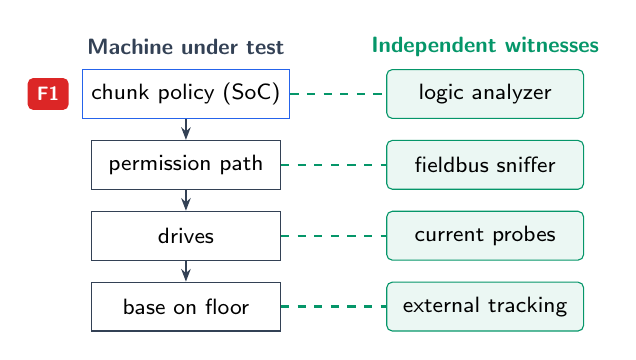
\begin{tikzpicture}[m/.style={draw=figslate, fill=white, minimum width=2.4cm, minimum height=0.62cm, font=\footnotesize, align=center}, w/.style={draw=figgreen, fill=figgreen!8, rounded corners=2pt, minimum width=2.5cm, minimum height=0.62cm, font=\footnotesize, align=center}, ar/.style={-{Stealth[length=1.6mm]}, figslate, thick}, tap/.style={dashed, figgreen, thick}]
        \node[font=\footnotesize\bfseries, text=figslate] at (0,2.95) {Machine under test};
        \node[m, draw=figblue] (soc) at (0,2.35) {chunk policy (SoC)};
        \node[m] (mcu) at (0,1.45) {permission path};
        \node[m] (drv) at (0,0.55) {drives};
        \node[m] (base) at (0,-0.35) {base on floor};
        \draw[ar] (soc) -- (mcu); \draw[ar] (mcu) -- (drv); \draw[ar] (drv) -- (base);
        \node[font=\scriptsize\bfseries, text=white, fill=figred, rounded corners=2pt] at (-1.75,2.35) {F1};
        \uncover<2->{
        \node[font=\footnotesize\bfseries, text=figgreen] at (3.8,2.95) {Independent witnesses};
        \node[w] (la) at (3.8,2.35) {logic analyzer};
        \node[w] (sn) at (3.8,1.45) {fieldbus sniffer};
        \node[w] (cp) at (3.8,0.55) {current probes};
        \node[w] (cam) at (3.8,-0.35) {external tracking};
        \draw[tap] (soc) -- (la); \draw[tap] (mcu) -- (sn); \draw[tap] (drv) -- (cp); \draw[tap] (base) -- (cam);}
      \end{tikzpicture}
    \end{column}
    \begin{column}{0.38\textwidth}
      \centering\safeimg[width=\textwidth,height=2.6cm,keepaspectratio]{saleae_logic8.jpg}\\[0.02cm]
      {\footnotesize A USB logic analyzer, one kind of external witness}\\[0.15cm]
      \small\uncover<3->{An on-board logger fails with the fault and shifts the timing it records.}
    \end{column}
  \end{columns}
  \mlsyscredit{Adversarial Verification, \S15.3 and figure 3 (simplified); probe effect: Gait 1986. Photo: Myself248, CC BY-SA 2.0, Wikimedia Commons (Saleae Logic8).}
  \note{[2 min] [CORE] Step 1: the machine under test, with F1 injected at the application processor. Step 2: every event the oracle scores is recorded by an instrument with its own clock and supply: a logic analyzer on dedicated trigger lines for the renewal, lease expiry, and stop command; a fieldbus sniffer for the delivered command; current probes for drive effort; external tracking cameras and encoders for base motion through standstill. A brake-switch contact confirms the holding brake but would miss the electric braking that starts first. The photo is a real logic analyzer board. Step 3: an on-board logging daemon cannot serve. A panicked kernel or saturated bus drops the very log it would write, and logging on the processor under test changes its timing: the probe effect, named by Gait in 1986. On-chip trace units and external analyzers observe without arbitrating. ENGAGE: why must the witness not share the machine's power rail? (Expected: an F4 sag would blind the witness at the moment it matters.) LINK: Lecture 4's independence requirement applies to the test bench too. WARN: a stop caused by a tripped thermal breaker looks like a pass if the oracle only checks distance; the witnesses must show the claimed path commanded the stop.}
\end{frame}

\begin{frame}{A late onset fails by \val{late_ms} ms while its travel passes by \val{late_rho_mm} mm}
  \centering
  \mlsyssteps[width=0.97\textwidth,height=6.4cm,keepaspectratio]{f1trace_step}{2}
  \mlsyscredit{Adversarial Verification, \S15.9.1 and figure 4 (model timelines; values from images/calcs.py).}
  \note{[2 min] [OPTIONAL] Step 1: the channels an F1 trial must witness, timed from the last valid renewal. The lease is high until it expires at \val{t_lease} ms; the permission tick commands the stop at \val{t_cmd} ms; the drive frame arrives at \val{t_frame}; deceleration must begin by \val{onset} ms, the green bound. Below, speed falls in an S-curve from \val{v_aisle} m/s to rest at \val{rest_on_time} ms, \val{travel_on_time} mm of travel. A refused probe replayed at \val{t_probe} ms tests that an expired lease cannot be renewed. Step 2: a trace that brakes at \val{onset_late} ms. The onset margin is minus \val{late_ms} ms. The base travels \val{stall_mm} mm further, \val{travel_late} mm, and keeps a margin of plus \val{late_rho_mm} mm against \val{f1_bound}. The verdict is FAIL, because a precommitted oracle checks both predicates. ENGAGE: the stop command issued on time; where would you look? (Expected: command delivery, the drive, or the brake; the lease check worked.) WARN: margins stay in their own units. Combining them requires scales fixed in advance; with the bounds as scales, minus \val{rho_onset_n} for onset and \val{rho_dist_n} for distance.}
\end{frame}

\begin{frame}{Diagnose: what verdict does each trial get?}
  \mlsysactivity{Diagnose}{2.5 min}
  \begin{columns}[T]
    \begin{column}{0.30\textwidth}
      \centering\safeimg[width=\textwidth,height=3.3cm,keepaspectratio]{nist_robot_test_bays.jpg}\\[0.02cm]
      {\footnotesize Robot test bays at NIST}
    \end{column}
    \begin{column}{0.68\textwidth}
      \small
      \textbf{1.} The injector dropped the fault frame before the transceiver.\enspace\uncover<2->{\textbf{\textcolor{figamber}{INVALID}}}\\[0.12cm]
      \textbf{2.} The logger crashed; the base stopped short of the rack.\enspace\uncover<2->{\textbf{\textcolor{figamber}{UNOBSERVABLE}}}\\[0.12cm]
      \textbf{3.} Onset at \val{chk_onset} ms, stop well short of the rack.\enspace\uncover<2->{\textbf{\textcolor{figred}{FAIL}}: $-\val{chk_rho}$~ms}\\[0.12cm]
      \textbf{4.} Both predicates held on independent witnesses.\enspace\uncover<2->{\textbf{\textcolor{figgreen}{PASS}}}\\[0.2cm]
      \uncover<3->{\footnotesize Unmeasured fields are recorded as unavailable, never as zero. INVALID and UNOBSERVABLE never become PASS and never leave the report.}
    \end{column}
  \end{columns}
  \mlsyscredit{Adversarial Verification, \S15.4.1 and Checkpoint 15.1 (\val{chk_onset} ms case: margin and \val{chk_extra} mm derived). Photo: NIST, public domain, Wikimedia Commons.}
  \note{[2.5 min] [CORE] The photo shows real test bays at NIST, where robot trials run under declared conditions. ENGAGE: pairs assign one of four verdicts to each trial, 90 seconds. Step 2: trial 1 is INVALID: the fixture failed to deliver the fault, so the machine was never tested; it is charged to the fixture. Trial 2 is UNOBSERVABLE: the scoring telemetry was lost; the partial trace is kept for diagnosis. Trial 3 is FAIL: the onset margin is minus \val{chk_rho} ms, \val{chk_extra} mm of extra travel before braking, and stopping short of the rack does not rescue it. Trial 4 is PASS only if preconditions were verified, every required witness was complete, and both margins are non-negative. Step 3: survivorship bias. The trials in which the logger crashes are often the most violent electrical transients, the ones most likely to hang the safety controller. Discarding them hides the failure under test. WARN: an aggregate of 98 percent over 5,000 trials says little if every trial ran at room temperature without contention; the campaign is judged by its weakest dimension. Land the segment: an oracle fixed in advance, scored from the event the fault disrupts, on witnesses the fault cannot reach.}
\end{frame}

% =============================================================================
% SECTION: FAULT LIST
% =============================================================================
\mlsysnote{[0.5 min] [CORE] Third segment: where the list of faults comes from. A second lecture on this chapter would end here.}
\mlsysdivider{Which faults should the campaign inject?}{Adversarial Verification, \S15.6}
\section{Fault List}

\begin{frame}{Deriving a fault list builds a five-element chain per fault}
  \centering
  \begin{tikzpicture}[c/.style={draw=figslate, fill=white, rounded corners=3pt, minimum width=2.6cm, minimum height=1.3cm, align=center, font=\footnotesize, text width=2.4cm, execute at begin node={\hyphenpenalty=10000\relax}}, ar/.style={-{Stealth[length=1.8mm]}, thick, figslate}]
    \node[font=\footnotesize\bfseries, anchor=west] at (-1.5,1.25) {Inverting a design record (F1)};
    \node[c, draw=figred] (a) at (0,0) {\textbf{Negated claim}\\renewal stops after lease issue};
    \node[c, right=0.32cm of a] (b) {\textbf{Injection point}\\kill the task, keep the timer};
    \node[c, right=0.32cm of b] (c) {\textbf{Detector}\\lease timer on the permission path};
    \node[c, right=0.32cm of c] (d) {\textbf{Response}\\revoke authority, resident stop};
    \node[c, right=0.32cm of d, draw=figgreen] (e) {\textbf{Pass condition}\\\val{onset} ms, \val{f1_bound} mm, witnessed};
    \draw[ar] (a) -- (b); \draw[ar] (b) -- (c); \draw[ar] (c) -- (d); \draw[ar] (d) -- (e);
    \uncover<2->{
    \node[font=\footnotesize\bfseries, anchor=west] at (-1.5,-1.25) {Working forward from physics (no record names these)};
    \node[c, draw=figamber, minimum height=0.9cm] at (0,-2.2) {brake lining glazes};
    \node[c, draw=figamber, minimum height=0.9cm] at (2.92,-2.2) {one supply chip resets both processors};
    \node[c, draw=figamber, minimum height=0.9cm] at (5.84,-2.2) {inverter noise on encoder lines};
    \node[c, draw=figamber, minimum height=0.9cm] at (8.76,-2.2) {drive keeps torque after a stop};
    \node[c, draw=figamber, minimum height=0.9cm] at (11.68,-2.2) {jumpered rack-end sensor};}
  \end{tikzpicture}
  \mlsyscredit{Adversarial Verification, \S15.6.1, \S15.6.2, and table 2; forward analysis after Leveson's STAMP and STPA (2011).}
  \note{[2.5 min] [CORE] Step 1: inversion. Take each recorded guarantee and negate it at its physical handoff. F1 negates ``the chunk policy renews within its lease.'' The chain has five elements: the negated condition; the physical injection point; the detector that must catch it; the bounded response; and the observable pass condition, scored on a witness. If any element cannot be defined or measured, the claim cannot be falsified: that is a verification gap, closed by new instrumentation, a narrower envelope, or a redesign. Step 2: inversion finds only faults someone wrote down. A second source works forward from the physical machine, following Leveson's systems-theoretic method: linings glaze under repeated stops, a shared power-management chip resets both processors in one droop, inverter switching couples into encoder lines, a shorted switch keeps producing torque after a stop command, and maintenance staff jumper a sensor. ENGAGE: which of the bottom row could a simulator that models ideal supplies ever produce? (Expected: none of the electrical ones.) LINK: compound faults come from Lecture 13's placement record: every resource the permission path shares with the learned workloads becomes a fault injected at the shared root. It also covers Lecture 14's single-writer handover handshake (A1 to A4).}
\end{frame}

\begin{frame}{The drive transient alone leaves \val{bus_margin} V above lockout}
  \begin{columns}[T]
    \begin{column}{0.36\textwidth}
      \begin{mlsyscard}{mlsysaccent}\footnotesize
        \textbf{Given}\\[0.05cm]
        Depleted bus \val{bus_low}~V; lockout \val{bus_uvlo}~V (datasheet)\\
        Source resistance \val{bus_r_mohm}~m$\Omega$; transient \val{i_rail}~A (illustrative)\\
        Permission-rail hold-up \val{holdup_s}~s (chosen)
      \end{mlsyscard}
    \end{column}
    \begin{column}{0.62\textwidth}
      \small
      \wstep{1}{Sag: $\val{bus_low} - \val{i_rail} \times \val{bus_r_ohm} = \val{bus_min}$~V, \textbf{\val{bus_margin}~V} above lockout}
      \wstep{2}{Lockout needs $(\val{bus_low} - \val{bus_uvlo})/\val{bus_r_ohm} = \textbf{\val{i_cross} A}$}
      \wstep{3}{So F4a must step the supply itself}
      \wstep{4}{F4b, flag to brakes set: \val{flag_to_set}~ms of \val{holdup_s}~s}
      \uncover<5->{\textcolor{figred}{Headroom vanishes near \val{r_cross}~m$\Omega$.}}
    \end{column}
  \end{columns}
  \mlsyscredit{Adversarial Verification, Napkin Math 15.2 (derived); recomputed in images/calcs.py.}
  \note{[2 min] [OPTIONAL] Worked example: Napkin Math 15.2, the compound fault on the shared drive bus. The drive bus feeds the traction drives directly and the application processor through a converter that locks out at \val{bus_uvlo} V; the permission path runs on an isolated, capacitor-backed rail. Step 1: at the depleted \val{bus_low} V point, a \val{i_rail} A drive transient through \val{bus_r_mohm} milliohms sags the bus to \val{bus_min} V, \val{bus_margin} V above lockout. Step 2: reaching lockout needs a \val{i_cross} A step, more than twice the transient. Step 3: so F4a cannot rely on the machine's own load; a programmable supply must step the bus while the processor runs at peak load, and the permission path must never reset. Step 4: F4b opens the permission rail's feed during the longest admitted stop: from the \val{ceiling_insp} m/s inspected-floor ceiling, flag to brakes set takes \val{flag_to_set} ms (\val{flag_path} ms of path, \val{holdup_stop} ms of jerk-limited stop, \val{engage} ms of brake engagement), leaving \val{holdup_margin} ms of the \val{holdup_s} s hold-up. ENGAGE: why open the feed during the longest stop rather than any stop? (Expected: a short stop passes on hold-up the claim never needed.) WARN: the \val{bus_r_mohm} milliohms is illustrative; at about twice that value the headroom disappears.}
\end{frame}

\begin{frame}{A printed patch turned a banana into a toaster at \val{patch_toaster} percent}
  \begin{columns}[c]
    \begin{column}{0.60\textwidth}
      \centering\safeimg[width=\textwidth,height=4.4cm,keepaspectratio]{brown2017_patch_fig1.png}
    \end{column}
    \begin{column}{0.38\textwidth}
      \small
      VGG16 sees a banana at \textbf{\val{patch_banana}\%}.\\[0.1cm]
      \uncover<2->{With a sticker on the table, it sees a toaster at \textbf{\textcolor{figred}{\val{patch_toaster}\%}}.\\[0.2cm]}
      \uncover<3->{The camera sends a well-formed, checksum-valid frame. Packet integrity says nothing about the scene.}
    \end{column}
  \end{columns}
  \mlsyscredit{Brown, Man\'e, Roy, Abadi, and Gilmer, ``Adversarial Patch,'' arXiv:1712.09665, 2017, Figure 1 (reproduced). Adversarial Verification, \S15.6.3.}
  \note{[2 min] [CORE] A published physical attack, Brown and colleagues, 2017. Step 1: a photo of a banana on a table goes to the VGG16 image classifier, which reports banana with \val{patch_banana} percent confidence. Step 2: the attackers print a patch, place it on the table, and photograph the scene again: toaster, \val{patch_toaster} percent. The patch works without access to the software, the bus, or the packets; it enters through the lens. Step 3: this is a transduction attack: the camera interface delivers a valid, on-time packet whose reading is false. Sun glare does the same by accident, and a laser can do it on purpose. ENGAGE: which check in the book's architecture could notice a well-formed frame of a false scene? (Expected: only a cross-sensor plausibility check or an independent witness; a checksum cannot.) WARN: students treat this as a software bug; the network did exactly what it was trained to do on the pixels it received.}
\end{frame}

\begin{frame}{Published attacks on robot proposers reached \val{pair_pct} percent}
  \begin{columns}[c]
    \begin{column}{0.52\textwidth}
      \centering{\footnotesize OpenVLA, patch in the camera's view}\\[0.02cm]
      \safeimg[width=\textwidth,height=5.0cm,keepaspectratio]{wang_patch.pdf}
    \end{column}
    \begin{column}{0.46\textwidth}
      \centering\safeimg[width=\textwidth,height=1.9cm,keepaspectratio]{unitree_go2.jpg}\\[0.05cm]
      \small
      \renewcommand{\arraystretch}{1.15}
      \begin{tabular}{@{}lcc@{}}\toprule
        \textbf{Harmful tasks} & \textbf{Direct} & \textbf{Jailbreak}\\\midrule
        Unitree Go2 & \val{go2_direct}/\val{robopair_n} & \textcolor{figred}{\textbf{\val{go2_pair}/\val{robopair_n}}}\\
        Jackal UGV & \val{jackal_direct}/\val{robopair_n} & \textcolor{figred}{\textbf{\val{jackal_pair}/\val{robopair_n}}}\\\bottomrule
      \end{tabular}
    \end{column}
  \end{columns}
  \mlsyscredit{Wang et al., ICCV 2025, arXiv:2411.13587, Table 1(a). Robey et al., ICRA 2025, arXiv:2410.13691, Tables 2, 3. Photo: HotNews Romania, CC BY 3.0, Commons.}
  \note{[2 min] [OPTIONAL] The proposer itself is an attack surface, through both of its inputs. Left: Wang and colleagues placed a small optimized patch in the camera view of OpenVLA, a \val{openvla_b}B vision-language-action model, on the four LIBERO simulated manipulation suites. Benign success was \val{wang_low} to \val{wang_high} percent; with the patch, success fell to \val{wang_patched} on every suite. Right: Robey and colleagues generated jailbreak prompts automatically (RoboPAIR) against language-model-controlled robots. Asked directly to perform harmful tasks, the Unitree Go2 robot dog complied in \val{go2_direct} of \val{robopair_n} trials and a Jackal ground robot with a GPT-4o planner in \val{jackal_direct} of \val{robopair_n}; with RoboPAIR prompts, both complied in \val{go2_pair} of \val{robopair_n}. The Go2 was attacked as a black box, a deployed commercial product. ENGAGE: on the running machine, where could such an input enter? (Expected: task instruction strings, floor placards, shipping labels, printed signs in the camera's view.) WARN: the patch results are in simulation; the jailbreak results are on real robots. Neither touched a wire.}
\end{frame}

\begin{frame}{How does the trial record a wrong-bin pick?}
  \mlsysactivity{Concept question}{2.5 min}
  \centering
  {\normalsize Speed, force, swept volume, freshness, and lease all pass,\\yet the item lands in the wrong bin. How is it recorded?}\\[0.35cm]
  \begin{minipage}{0.86\textwidth}\small
    \choice{A}{PASS: no monitored limit was breached}\\[0.1cm]
    \choice{B}{FAIL: the enforcer should have refused it}\\[0.1cm]
    \answerat{2}{C}{Physical predicates pass; the wrong action is a coverage deficit, never a pass}
  \end{minipage}\\[0.3cm]
  \uncover<2->{\footnotesize The permission path checks physical limits and cannot read meaning. It clamps any breach within \val{enforcer_deadline}~$\mu$s.}
  \mlsyscredit{Adversarial Verification, \S15.6.3 and table 2 (proposer-injection row); Lecture 10 (admission checks physics and leaves meaning to the proposer).}
  \note{[2.5 min] [CORE] Peer instruction: vote, discuss with a neighbor for one minute, vote again. Step 2: C. The permission path does not read the task instruction or the intent model's candidate set; it checks velocity and torque envelopes, stopping reserve, swept-volume occupancy, evidence freshness, and lease validity, and it clamps or refuses any proposal that breaches one within its \val{enforcer_deadline} microsecond deadline. A wrong action inside every limit is admitted. A is wrong because it would credit the proposer-injection case with a pass it did not earn. B is wrong because no physical check was violated; Lecture 10 showed that admission checks physics and cannot check meaning, and Lecture 1's proposal boundary puts semantic correctness on the proposer's side. The campaign scores proposer attacks only against the physical oracle and records the wrong action as a semantic coverage deficit. ENGAGE: what claim would extend the result to every possible proposal? (Expected: an architectural or formal argument that no source can bypass the permission path.) Land the segment: faults come from inverting records, from physics, from shared resources, and from attacks on the proposer's inputs.}
\end{frame}

% =============================================================================
% SECTION: LADDER
% =============================================================================
\mlsysnote{[0.5 min] [CORE] Fourth segment: where each trial runs, and how to search beyond the first one. A second lecture on this chapter would start here.}
\mlsysdivider{Which test bench can show which failure?}{Adversarial Verification, \S15.7 to \S15.9}
\section{Ladder}

\begin{frame}{Each qualification rung makes another part of the loop real}
  \centering
  \mlsyssteps[width=0.97\textwidth,height=4.8cm,keepaspectratio]{ladder_step}{4}\\[0.05cm]
  {\footnotesize Ladder cells, green: real item.\enspace Dashed: model.\enspace SIL, PIL, HIL: software, processor, hardware in the loop.}
  \mlsyscredit{Adversarial Verification, \S15.7.1, figure 2, and table 3, redrawn at slide size.}
  \note{[2.5 min] [CORE] The qualification ladder orders four environments by how much of the loop is physical. Step 1: software in the loop runs the decision logic on a workstation; drives and floor are models; execution timing, bus timing, and supply transients are absent. It can sweep millions of variations in parallel. Step 2: processor in the loop runs the compiled enforcer on its real target chip, so instruction timing and stack headroom are real; the bus is a model. Step 3: hardware in the loop adds the real fieldbus, regulators, and drive stages, against a real-time plant model or a dynamometer; only floor contact is a model; it runs in real time. Step 4: the physical rig adds the production chassis, brakes, harness, and floor; throughput is limited by resets and wear. A mechanism can fail only on a rung that contains it: a simulator with stiff supplies cannot sag the bus of F4. That is the digital twin delusion: a simulator never compared with a measured stop of this machine is only a model of it. WARN: higher rungs do not subsume lower ones; agreement between two rungs supports only the mechanisms both contain. Trace replay and shadow operation break the loop entirely, because the candidate's commands never change what it sees next.}
\end{frame}

\begin{frame}{Which rung first contains F2, F3, and a jam?}
  \mlsysactivity{Predict}{2.5 min}
  \begin{columns}[T]
    \begin{column}{0.48\textwidth}
      \centering
      \safeimg[width=\textwidth,height=1.9cm,keepaspectratio]{sail_payload_bay.jpg}\\[0.01cm]
      {\footnotesize HIL: NASA avionics integration lab}\\[0.05cm]
      \safeimg[width=\textwidth,height=1.8cm,keepaspectratio]{chassis_dyno_opel.jpg}\\[0.01cm]
      {\footnotesize Rig: a car on a chassis dynamometer}
    \end{column}
    \begin{column}{0.50\textwidth}
      \small
      \textbf{F2:} a frame held at the image processor\\
      \uncover<2->{\textcolor{figgreen}{\textbf{HIL:}} the real camera link and processors.\\[0.12cm]}
      \textbf{F3:} fieldbus frames lost at a drive\\
      \uncover<2->{\textcolor{figgreen}{\textbf{HIL:}} the real transceivers and bus. PIL uses a debug port.\\[0.12cm]}
      \textbf{Jam:} a seized wheel bearing\\
      \uncover<2->{\textcolor{figgreen}{\textbf{Physical rig:}} the yaw it causes depends on real floor contact.}
    \end{column}
  \end{columns}
  \mlsyscredit{Adversarial Verification, Checkpoint 15.2. Photos: NASA/Smiley N. Pool, public domain; Tupungato, CC BY 3.0; Commons.}
  \note{[2.5 min] [CORE] Two real rungs. Top: NASA's Shuttle Avionics Integration Laboratory, a skeletal avionics version of the orbiter that ran actual orbiter hardware and flight software, the wiring of its simulated payload bay in 2011. Bottom: a car on a chassis dynamometer, rolling-road testing at an Opel factory; a physical rig drives real wheels against a load. ENGAGE: for each fault, pick the lowest rung that contains its causal mechanism, one minute. Step 2: F2 needs the real camera serial link, image processor, and processors under load: HIL, with an inline interposer that holds a frame while keeping its timestamp. F3 needs real transceivers and bus timing: HIL; processor in the loop routes I/O over a debug interface and cannot stress the bus. The jam's pass condition is that the base stays inside its \val{side_clearance} m side clearance while one wheel is blocked; the yaw comes from tire contact, so it needs the physical rig, with a wheel clamp. WARN: students pick software in the loop for F2 because it is a timing fault; the delay hides in buffers that only exist on the real hardware.}
\end{frame}

\begin{frame}{Proof reaches the permission path; the \val{intent_b}B proposer is too large}
  \begin{columns}[c]
    \begin{column}{0.60\textwidth}
      \centering\safeimg[width=\textwidth,height=5.4cm,keepaspectratio]{vnn.pdf}
    \end{column}
    \begin{column}{0.38\textwidth}
      \small
      The largest network scored in the 2025 verification competition: \textbf{\val{vnn_max_m}M} parameters.\\[0.15cm]
      \uncover<2->{The intent model is \textbf{\val{intent_over_vnn} times} larger, and both proposers read an unbounded camera stream.\\[0.15cm]}
      \uncover<3->{Proof goes to the compact permission path; the proposers are tested.}
    \end{column}
  \end{columns}
  \mlsyscredit{Kaulen et al., VNN-COMP 2025, arXiv:2512.19007, Table 3. Running machine: Adversarial Verification, \S15.7.3. Ratio derived.}
  \note{[2 min] [OPTIONAL] Formal proof is a fifth source of evidence, and it holds only inside its model of the plant. Step 1: each dot is the largest network in one of the \val{vnn_n} benchmarks scored at the 2025 International Verification of Neural Networks Competition; the largest is VGGNet16 at \val{vnn_max_m} million parameters. Complete verifiers such as alpha-beta-CROWN prove that every input in a bounded set, for example every image within a small pixel perturbation, gives an acceptable output. Step 2: the running machine's intent model has \val{intent_b} billion parameters, \val{intent_over_vnn} times the largest. The \val{chunk_m} million parameter chunk policy is within that range by size, but no proof covers its input: a changing stream of high-resolution frames has no bounded set that implies stopping safety. Closed-loop reachability tools work for small controllers and low-dimensional plants. Step 3: so the design puts proof on the deterministic permission path, which reads a handful of calibrated measurements and enforces a stopping invariant a proof can reach; that is Lecture 8's third law, proposal is not permission, seen from the verifier's side. ENGAGE: what premises does a proof of the permission path leave to physical test? (Expected: plant dynamics, observation deadlines, bus latencies, torque limits.)}
\end{frame}

\begin{frame}{Signed robustness turns testing into a search for the worst case}
  \begin{columns}[c]
    \begin{column}{0.54\textwidth}
      \centering\mlsyssteps[width=\textwidth,height=5.7cm,keepaspectratio]{stl_step}{2}
    \end{column}
    \begin{column}{0.44\textwidth}
      \small
      $\rho\,(\text{always } \varphi) = \min_t \rho(\varphi, t)$\\[0.05cm]
      {\footnotesize $\rho$: signed margin of a trace against a temporal requirement $\varphi$}\\[0.2cm]
      \uncover<2->{Falsification: choose the start state and disturbance that \textbf{minimize} $\rho$, within what a test bench can deliver.\\[0.15cm]}
      \uncover<3->{\footnotesize A search that finds no violation certifies nothing.}
    \end{column}
  \end{columns}
  \mlsyscredit{Adversarial Verification, \S15.9.1 and \S15.9.2 (signal temporal logic: Maler and Nickovic 2004; robustness: Fainekos and Pappas 2009). Traces illustrative.}
  \note{[2.5 min] [CORE] A PASS or FAIL tells a search nothing about how close a trial came. Signal temporal logic writes requirements over continuous signals, such as ``always keep clearance,'' and returns a signed margin. Step 1: for ``always,'' the margin is the worst point along the trace: the solid trace keeps 0.15 m at its closest point, a pass with 15 cm to spare. Step 2: the dashed trace dips 0.04 m below the limit, a violation of depth 4 cm. Because the margin is a number, an optimizer can drive it down: this is falsification, the physical counterpart of an adversarial example, searching over initial speed, payload, friction, and disturbance waveforms. The disturbance must be smooth and bounded, because a test bench cannot deliver a spike faster than its slew rate; a synthesized counterexample the fixture cannot reproduce is INVALID on hardware. Tools: S-TaLiRo and Breach; CMA-ES or Bayesian optimization when each physical trial is expensive. Step 3: a found violation refutes the claim; an empty search leaves the unsearched space open. ENGAGE: why keep F1's onset deadline outside the formula? (Expected: time and space margins have different units; the onset is a scalar check on reaction time.)}
\end{frame}

\begin{frame}{A simulated margin counts only after the transfer discount}
  \begin{columns}[c]
    \begin{column}{0.48\textwidth}
      \centering
      {\Large $\rhophys \;\ge\; \rhosim - L\,\Delta$}\\[0.25cm]
      {\footnotesize $\Delta$: largest gap between simulated and measured trajectories over the envelope\\$L$: how fast the margin degrades per unit of that gap}\\[0.3cm]
      \small\uncover<2->{Rack end, $L = 1$~m per unit: a simulated \val{spare}~mm reserve guarantees a physical margin only if $\Delta < \textbf{\val{eps_gap_max}}$.}
    \end{column}
    \begin{column}{0.50\textwidth}
      \centering\safeimg[width=\textwidth,height=3.6cm,keepaspectratio]{iihs_tucson_crash.jpg}\\[0.02cm]
      {\footnotesize A physical crash test at the IIHS}
    \end{column}
  \end{columns}
  \mlsyscredit{Adversarial Verification, \S15.9.4, equation 6 (derived). Photo: Brady Holt, CC BY 3.0, Wikimedia Commons.}
  \note{[2 min] [CORE] Simulation is where search is cheap, so its margins must be translated. Delta is the largest gap between simulated and physical trajectories under matched conditions, in a predeclared normalized norm; L is the Lipschitz constant, how much the clearance margin can change per unit of that gap. The physical margin is at least the simulated margin minus L times Delta. Step 2: for the rack end, with position normalized by 1 m and unit weight, L is 1 m per unit. A simulated stop that keeps the whole \val{spare} mm reserve guarantees a positive physical margin only if Delta is below \val{eps_gap_max}, a position error under \val{spare_mm0} mm. A simulator validated to a few centimeters transfers most of its margin; one never compared with a measured stop transfers none. The photo is the point: only physical tests, like this crash test at the Insurance Institute for Highway Safety, measure Delta. LINK: measuring it reuses Lecture 6's paired probing, with excitation at full-rate deceleration and external instruments. WARN: a Delta measured on an unloaded, cool machine does not cover a loaded, throttled one. Land the segment: choose the rung that contains the mechanism, search for small margins, and discount simulated ones.}
\end{frame}

% =============================================================================
% SECTION: EVIDENCE
% =============================================================================
\mlsysnote{[0.5 min] [CORE] Last segment: how many trials, what statistics they support, and the record that carries them to release.}
\mlsysdivider{How much evidence does a rate claim need?}{Adversarial Verification, \S15.10 and \S15.11}
\section{Evidence}

\begin{frame}{How many zero-miss injections prove \val{fit_target} FIT?}
  \mlsysactivity{Estimate}{3 min}
  \begin{columns}[T]
    \begin{column}{0.38\textwidth}
      \begin{mlsyscard}{mlsysaccent}\footnotesize
        \textbf{Given} (illustrative; 1 FIT $=$ 1 fault per $10^9$ hours)\\[0.05cm]
        Sensors \val{fit_sensors}; compute \val{fit_compute}; transceivers and power \val{fit_power}; gate drivers \val{fit_gate} FIT\\
        Unmitigated target \val{fit_target} FIT, \val{confidence_pct}\% confidence (chosen)
      \end{mlsyscard}
    \end{column}
    \begin{column}{0.60\textwidth}
      \small
      \wstep{1}{Raw rate: \textbf{\val{fit_raw} FIT}}
      \wstep{2}{Coverage: $1 - \val{fit_target}/\val{fit_raw} = \textbf{\val{cov_pct}\%}$}
      \wstep{3}{Zero misses: $n \ge \ln \val{miss_confidence} / \ln \val{cov_frac} = \val{n_exact}$, so \textbf{\val{n_cov}} (rule of three: \val{rule3})}
      \wstep{4}{{\normalsize Your turn: a \val{fit_target_tight} FIT target?}\enspace\uncover<5->{\textbf{\textcolor{figred}{\val{cov_tight_pct}\%, \val{n_cov_tight} injections}}}}
      \uncover<5->{\footnotesize Sample in proportion: \val{n_gate} of \val{n_cov} hit gate drivers.}
    \end{column}
  \end{columns}
  \mlsyscredit{Adversarial Verification, Napkin Math 15.3 (derived); zero-failure bound from Lecture 7. Recomputed in images/calcs.py.}
  \note{[2.5 min] [CORE] Worked example and estimate, Napkin Math 15.3. FIT is failures in time, one per billion operating hours. Step 1: the four component strata sum to \val{fit_raw} FIT. Step 2: to leave at most \val{fit_target} FIT unmitigated, diagnostic coverage, the rate-weighted fraction of faults whose effect is caught, must be \val{cov_pct} percent. Step 3: each injection misses with probability 1 minus coverage; zero misses in n trials bounds that at \val{confidence_pct} percent confidence when n is at least ln \val{miss_confidence} over ln \val{cov_frac}, \val{n_cov}. Lecture 7's rule of three gives \val{rule3}. Step 4: students compute the \val{fit_target_tight} FIT case, 60 seconds. Step 5: \val{cov_tight_pct} percent and \val{n_cov_tight} injections. A tenfold tighter target costs tenfold more trials; the length of the fault list does not set the campaign size. WARN: the count holds only if injections are drawn in proportion to the rates, \val{n_gate} to gate drivers, \val{n_power} to transceivers and power, \val{n_sensors} to sensors, and \val{n_compute} to compute; uniform injection tests a different distribution. Repeated hot stops also couple trials through winding and lining heat. LINK: Lecture 7's exposure wall says fleet hours cannot replace this: bounding $10^{\val{wall_rate_exp}}$ per hour needs about $\val{wall_bh} \times 10^9$ failure-free hours, and they count only for the configuration that logged them.}
\end{frame}

\begin{frame}{Weighting runs near failure cuts the runs about $\val{is_speedup_mant} \times 10^{\val{is_speedup_exp}}$ times}
  \centering
  \mlsyssteps[width=0.86\textwidth,height=4.1cm,keepaspectratio]{is_ladder_step}{3}\\[0.1cm]
  {\small One rare-event rate: a delay past the \val{t_spare} ms spare, $p = \val{p_fail_mant} \times 10^{\val{p_fail_exp}}$ per stop (illustrative).}\\[0.05cm]
  \uncover<3->{\footnotesize Runs weighted by $p(x)/q(x)$: \val{q_fail_pct}\% fail, yet the estimate stays $\val{p_fail_mant} \times 10^{\val{p_fail_exp}}$.}
  \mlsyscredit{Adversarial Verification, \S15.10.2 and its figure (exponential delay, mean \val{is_mean} ms; \val{rel_err_pct} percent relative error; cross-entropy proposal). Recomputed in images/calcs.py.}
  \note{[2 min] [CORE] Worked example: estimating one rare rate. The model: queue delays are exponential with mean \val{is_mean} ms, an illustrative assumption; a delay beyond \val{t_spare} ms spends the spare, probability $\val{p_fail_mant} \times 10^{\val{p_fail_exp}}$ per stop. Step 1: plain Monte Carlo needs about $\val{n_mc_mant} \times 10^{\val{n_mc_exp}}$ runs to estimate it to \val{rel_err_pct} percent, because almost every run ends in a safe stop. Step 2: a zero-failure campaign needs $\val{n_zero_mant} \times 10^{\val{n_zero_exp}}$ runs just to bound it. Step 3: importance sampling draws from a proposal q that puts runs near failure, then weights each run by the likelihood ratio, the operational density over the proposal density, to recover an unbiased estimate. The cross-entropy method finds q in \val{n_levels_words} steps (levels \val{ce_level1}, \val{ce_level2}, \val{ce_level3}, then \val{ce_level4} ms; final mean \val{ce_mean} ms). \val{n_is} runs suffice. WARN: \val{q_fail_pct} percent of proposal runs fail, and that fraction says nothing about real frequency; the same holds for falsification runs, which carry no weights at all. A rate belongs in a safety case only with its declared model, proposal, and weights. ENGAGE: what happens if the proposal misses a failure path entirely? (Expected: the estimate is biased low, with deceptively small variance, and no diagnostic sees it.)}
\end{frame}

\begin{frame}{Cross-entropy sampling cut error most at the rarest threshold}
  \begin{columns}[c]
    \begin{column}{0.56\textwidth}
      \centering\safeimg[width=\textwidth,height=5.8cm,keepaspectratio]{okelly.pdf}
    \end{column}
    \begin{column}{0.42\textwidth}
      \small
      \val{ok_runs} runs with a learned proposal against \val{ok_runs} plain runs, collision-risk events near $10^{\val{ok_event_exp}}$.\\[0.2cm]
      \uncover<2->{The gain shrinks as events become common.\\[0.2cm]}
      \uncover<3->{\footnotesize Check the weights: the effective sample size of the model's \val{n_is} runs is about \textbf{\val{ess}}.}
    \end{column}
  \end{columns}
  \mlsyscredit{O'Kelly et al., NeurIPS 2018, arXiv:1811.00145, Table 1 (relative error derived). ESS: Adversarial Verification, \S15.10.2.}
  \note{[2 min] [OPTIONAL] Published measurements. O'Kelly and colleagues estimated rare dangerous-event probabilities for an autonomous-driving policy in simulation with the cross-entropy method. Step 1: relative standard error, computed from their Table 1, for \val{ok_runs} naive runs, \val{ok_runs} cross-entropy runs, and a \val{ok_big_runs_m} million run naive baseline, at four danger thresholds. At the rarest threshold, about $10^{\val{ok_event_exp}}$, cross-entropy cut the relative error from \val{ok_rse_naive} to \val{ok_rse_ce} percent; the paper reports \val{ok_vr_low} to \val{ok_vr_high} times variance reduction across the thresholds of its Figure 2. Step 2: at the most common threshold, the naive estimate was as good. Real stacks depart from the clean exponential model; the gain is real but smaller. Step 3: the weight diagnostic. The effective sample size, the square of the sum of the weights over the sum of their squares, is about \val{ess} for the model's \val{n_is} runs; a value near 1 would mean a few heavy weights carry the estimate. ENGAGE: why can the effective sample size look healthy while the estimate is wrong? (Expected: it measures weight concentration and cannot show whether the proposal covers every failure region.)}
\end{frame}

\begin{frame}{A fitted tail endpoint certifies no physical stop}
  \begin{columns}[c]
    \begin{column}{0.56\textwidth}
      \centering\safeimg[width=\textwidth,height=5.8cm,keepaspectratio]{evt.pdf}
    \end{column}
    \begin{column}{0.42\textwidth}
      \small
      Extreme value theory fits only the exceedances past a high threshold.\\[0.15cm]
      Tail shape $\xi$: heavy ($>0$), exponential ($=0$), or bounded ($<0$).\\[0.15cm]
      \uncover<2->{F1 has zero physical trials, so it supports no tail fit at all. The reserve is \val{spare_left}~mm after allocation.}
    \end{column}
  \end{columns}
  \mlsyscredit{Adversarial Verification, \S15.10.3 (generalized Pareto distribution; Coles 2001). Curves illustrative, scale 10 mm.}
  \note{[1.5 min] [OPTIONAL] Rates say how often; tails say how far. Extreme value theory fits the exceedances above a high threshold with a generalized Pareto distribution. Step 1: three shapes. A positive shape parameter gives a heavy tail; zero, exponential; negative, a bounded tail with a finite endpoint, the dotted line. The endpoint is a property of the fitted curve and certifies no stop; a filter's containment is verified by testing its premises and latencies. Fitting to unweighted falsification runs models the optimizer's search instead of the plant; the runs need the importance weights. A simulated return level must also add the transfer discount before it is compared with the reserve: \val{spare} mm at the ceiling, \val{spare_left} mm once the dispatch-to-admission allocation is charged. Step 2: when a fault mode has no measured physical trials, as F1 has none in the book, there is nothing to fit. ENGAGE: what does a fit with a positive shape demand of the team? (Expected: find what drives the heavy tail: the threshold choice, sensor noise, or unmodeled delays.)}
\end{frame}

\begin{frame}{The fault-record set binds each trace to its claim and its gaps}
  \begin{columns}[T]
    \begin{column}{0.48\textwidth}
      \small
      \textbf{Header:} trial, claim, envelope point, injection, oracle digest\\[0.05cm]
      \textbf{Outcome:} latencies, signed margins, verdict, bundle digest\\[0.05cm]
      \textbf{Set adds:} rung coverage, transfer bounds, tail estimates, \textcolor{figred}{coverage deficits}, signatures
    \end{column}
    \begin{column}{0.50\textwidth}
      {\footnotesize\textbf{The planned F1 header, signed (our run)}}\\[0.05cm]
      \begin{logblock}[6.8]
"trial\_id": "F1-restricted-001",\\
"envelope": \{"speed\_mps": 1.0, "payload\_kg": 50,\\
\hspace*{2em}"floor\_mu": 0.12\},\\
"injection": \{"mode": "kill chunk-policy task",\\
\hspace*{2em}"timer\_isr": "left running"\},\\
"oracle\_sha256": "d4d546c7400e37e94128f0cc...",\\
\textcolor{figred}{"outcome": \{"trials": "unavailable",}\\
\textcolor{figred}{\hspace*{2em}"max\_onset\_ms": "unavailable", ...\},}\\
"verdict": null\\
signature\_ed25519: b1f0b3e9c142e5181ed9...
      \end{logblock}
    \end{column}
  \end{columns}
  \mlsyscredit{Adversarial Verification, \S15.4.2, \S15.11. Our run: images/make\_record.py (SHA-256; demonstration Ed25519 key).}
  \note{[2 min] [CORE] The record this lecture adds to the chain, the fault-record set. Left: each fault record binds a signed header to the independently retained trace. Identity fields name the trial, the claim, the envelope point, the injection, and a digest of the oracle fixed before the run; outcome fields hold the measured latencies, the signed margins, the four-state verdict, and a digest of the evidence bundle. The set adds the per-rung coverage of the ladder, the sim-to-real transfer bounds, any tail estimates with their weights, the explicit list of coverage deficits, and multi-party signatures. Right: we built the planned F1 header with the chapter's values and signed it: the restricted point, \val{v_restricted} m/s with \val{payload} kg on a \val{mu_insp} floor, and the oracle of \val{onset} ms and \val{f1_restricted} mm hashed with SHA-256. The outcome fields say ``unavailable,'' because the book has run no trial, and the verdict is empty. A missing value is never a zero. ENGAGE: why sign the oracle before the run? (Expected: so nobody can relax a threshold after seeing the trace.) WARN: a signature proves who recorded the evidence; sufficiency needs its own argument.}
\end{frame}

\begin{frame}{The fault-record set is the thirteenth record in the chain}
  \centering
  \mlsyskitfig[width=0.92\textwidth,height=5.2cm,keepaspectratio]{record_chain_l15}
  \mlsyscredit{The record chain, The Causal Boundary, \S1.11.}
  \note{[0.5 min] [CORE] NARRATE: Lecture 1's record chain with today's record lit. The fault-record set comes after Lecture 14's authority record and before the release manifest; it consumes the authority, placement, enforcement, and evaluation records. The records after it are still dimmed. FLEX: [CORE].}
\end{frame}

\begin{frame}{Are these two claims true or false?}
  \mlsysactivity{Concept question}{2 min}
  \small
  \textbf{1.} Independent watchdogs on each task guarantee the end-to-end deadline.\\[0.05cm]
  \uncover<2->{\textcolor{figred}{\textbf{False.}} An unmonitored queue can age the evidence while every task meets its slice. At \val{v_aisle}~m/s a \val{t_spare}~ms wait in it spends the whole spare.\\[0.3cm]}
  \textbf{2.} A trial whose logger crashed while the base stopped short is evidence of safety.\\[0.05cm]
  \uncover<3->{\textcolor{figred}{\textbf{False.}} It is UNOBSERVABLE. The violent transients that crash loggers are the ones most likely to hang the controller; the aisle has no end stop like the test cell's.}
  \mlsyscredit{Adversarial Verification, \S15.12 (fallacies; \val{t_spare} ms derived in images/calcs.py).}
  \note{[2 min] [CORE] The chapter's two fallacies as true or false; students vote on each. Step 2: false. A perception front end, the chunk policy, and the permission monitor can each meet their local slice while an unmonitored queue between them holds stale observations; every local watchdog reports healthy. The importance-sampling example priced this queue: at \val{v_aisle} m/s it exhausts the \val{spare} mm spare after \val{t_spare} ms, and after \val{t_left} ms once Lecture 13's dispatch-to-admission allocation is charged. The countermeasure is a capture-to-torque age check: compare the capture timestamp with the monitor's decision tick. Step 3: false. Ground bounce and inductive kicks from high-energy faults crash loggers and overflow frame grabbers; those are the trials most likely to leave the safety controller hung in an exception handler. The test cell has an end stop; the warehouse aisle does not. Report all four verdict counts, and investigate why the witness failed before repeating the trial. ENGAGE: which earlier slide's watchdog was task-blind? (Expected: watchdog A in our run.)}
\end{frame}

% =============================================================================
% CLOSE
% =============================================================================
\begin{frame}{Which test would settle the Toyota question?}
  \mlsysactivity{Retrieval}{2.5 min}
  \begin{columns}[c]
    \begin{column}{0.28\textwidth}
      \centering\safeimg[width=\textwidth,height=2.6cm,keepaspectratio]{camry_2005.jpg}
    \end{column}
    \begin{column}{0.70\textwidth}
      \small
      \only<1|handout:0>{{\normalsize Write the claim, the injection, the detector, the witness, and the oracle.}}
      \only<2->{\renewcommand{\arraystretch}{1.0}\begin{tabular}{@{}l>{\raggedright\arraybackslash}p{8.3cm}@{}}\toprule
        Claim & a dead throttle task leads to a safe throttle state\\
        Injection & kill the task; keep the timer interrupt alive\\
        Detector & watchdog fed by task progress\\
        Witness & throttle position measured outside the controller\\
        Oracle & idle within a deadline fixed before the run\\
        \textcolor{figred}{Also} & \textcolor{figred}{fault the shared pedal converter for both processors}\\\bottomrule
      \end{tabular}}
    \end{column}
  \end{columns}
  \mlsyscredit{Adversarial Verification, War Story 15.1 (Barr 2013; Dunn 2013). Photo: Brad E. Williams, public domain, Wikimedia Commons.}
  \note{[2.5 min] [CORE] Synthesis: back to the hook with today's vocabulary. Give 60 seconds to write the five-element chain. Step 2: the claim is that the system reaches a safe throttle state when the control task dies. The injection is exactly F1's: terminate the task or freeze its output while the timer interrupt keeps running. The detector under test is whatever feeds the watchdog; only a progress check can notice. The witness measures throttle position and engine response outside the controller, on its own clock and supply. The oracle states the deadline to idle before the run. The record answers a second question the design rule alone does not raise: the monitor processor read the same pedal converter, so the campaign must inject faults at that shared input too. The book treats the task-blind mechanism as an attributed hypothesis; this test is how a team would settle it for its own machine. The lecture's claim in one line is that the claims that matter describe behavior after a fault, and only a precommitted, witnessed injection tests them.}
\end{frame}

\begin{frame}{Takeaways}
  \thumbline{thumb_corner_step2.pdf}{A claim holds over a declared envelope that includes the machine's own state; \val{v_aisle}~m/s on a \val{mu_insp} floor needs \val{budget_insp_m}~m.}\\[0.12cm]
  \thumbline{thumb_refevents_step3.pdf}{An oracle is fixed before the run and scored from the event the fault disrupts: F1 is \val{onset}~ms and \val{f1_bound}~mm from renewal.}\\[0.12cm]
  \thumbline{thumb_wang_patch.pdf}{Faults come from inverted records, physics, shared resources, and attacks; a wrong action inside the limits is a deficit.}\\[0.12cm]
  \thumbline{thumb_ladder_step4.pdf}{A mechanism fails only on a rung that contains it; simulated margins count after the transfer discount.}\\[0.12cm]
  \thumbline{thumb_is_ladder_step3.pdf}{A \val{fit_target} FIT target needs \val{n_cov} zero-miss injections; rates need weights, and the record keeps every gap.}
  \note{[1 min] [CORE] One line per segment, with the last two lines splitting the final segment. Ask students which slide taught each line. If short on time, read the second and the fifth.}
\end{frame}

\begin{frame}{Open questions}
  \begin{columns}[c]
    \begin{column}{0.64\textwidth}
      \small
      \begin{itemize}\setlength{\itemsep}{0.12cm}
        \item A proposer update changes behavior everywhere. Which fault records stay valid, and who decides?
        \item A transduction attack and sun glare produce the same packet. Should the campaign test them as one fault or two?
        \item How small must a simulator's transfer gap be before a regulator should accept its sweeps as evidence?
      \end{itemize}
    \end{column}
    \begin{column}{0.34\textwidth}
      \centering\safeimg[width=\textwidth,height=3.2cm,keepaspectratio]{tin_whisker_esa.jpg}\\[0.02cm]
      {\footnotesize Physics adds faults no design record lists}
    \end{column}
  \end{columns}
  \mlsyscredit{Photo: European Space Agency, CC BY-SA 3.0 IGO, Wikimedia Commons.}
  \note{[0.5 min] [OPTIONAL] No single answer. Pick one for discussion or assign one as a short written response. The first previews Lecture 16's safety case. The second contrasts intent with mechanism: the same detector and oracle may serve both, but the injection rig differs. The third asks for a number students can defend, given the \val{spare} mm reserve and the transfer discount.}
\end{frame}

\begin{frame}{Read and explore}
  \small
  \begin{itemize}\setlength{\itemsep}{0.03cm}
    \item \textbf{Read:} Adversarial Verification, \S15.1 to \S15.13; Checkpoints 15.1 to 15.3; Napkin Math 15.1 to 15.3 by hand.
    \item Arlat et al., ``Fault Injection for Dependability Validation,'' \emph{IEEE TSE}, 1990.
    \item Leveson, \emph{Engineering a Safer World}, MIT Press, 2011.
    \item Fainekos and Pappas, ``Robustness of Temporal Logic Specifications,'' \emph{TCS}, 2009.
    \item Corso et al., ``A Survey of Algorithms for Black-Box Safety Validation,'' \emph{JAIR}, 2021.
    \item Kochenderfer, Katz, Corso, and Moss, \emph{Algorithms for Validation}, MIT Press, 2026.
  \end{itemize}
  \note{[0.5 min] [CORE] The chapter first, with its three checkpoints and three worked examples. Arlat and colleagues made fault injection an experimental method: faults, workload, readouts, measures, the template for today's record. Leveson's systems-theoretic method is the forward hazard analysis of the Fault List segment. Fainekos and Pappas define the signed robustness used in search. Corso and colleagues survey falsification, most-likely failures, and rare-event estimation. Kochenderfer and colleagues collect these algorithms in one textbook. FLEX: add the lab your course uses for hardware-in-the-loop testing.}
\end{frame}

\begin{frame}[c]
  \begin{columns}[c]
    \begin{column}{0.34\textwidth}
      \centering\mlsyskitfig[width=\textwidth,height=2.2cm,keepaspectratio]{thumb_record_chain}
    \end{column}
    \begin{column}{0.62\textwidth}
      {\small\textcolor{lightgray}{NEXT LECTURE \textbar{} DEPLOYMENT RELEASE}}\\[0.5cm]
      {\LARGE\bfseries Why can a machine that passes every trial still lack the evidence to work among people?}
    \end{column}
  \end{columns}
  \note{[0.5 min] [CORE] Today produced fault records with verdicts, coverage, and gaps. None of them decides whether the machine may operate. Lecture 16 joins them with the authority, placement, and evaluation records in a safety case, states which claims the evidence supports, refuses where a premise is unknown, and sets the conditions under which permission lapses. The next record in the chain is the release manifest.}
\end{frame}

\end{document}
